%!TEX program = xelatex
%%%%%%%%%%%%%%%%%%%%%%%这是导言部分的开始%%%%%%%%

%========= 导言部分声明文档的类型=================
\documentclass{article}

%=========导言部分可可以加载宏包=================
\usepackage{amsmath}                % 数学公式排版宏包
\usepackage{amssymb}                % 数学符号命令宏包
\usepackage{amsthm}                 % 数学定理宏包
\usepackage[UTF8]{ctex}             % 中文输入宏包
\usepackage[a4paper]{geometry}      % 页面设置宏包
\usepackage{setspace}               % 行间距宏包
\usepackage{graphicx}               % 图片宏包
\usepackage{listings}               % 代码宏包
\usepackage{color}					% 颜色宏包
\usepackage{xcolor}                 % 颜色处理宏包
\usepackage{float}                  % 浮动对象式样宏包
\usepackage{fontspec}
\usepackage{enumerate}				% 列举编号包

%=========页面设置==============================
\geometry{left=1cm,right=1cm,top=1cm,bottom=2cm}
\onehalfspacing
\setlength\parindent{0em}

%=========代码格式设置============================
\definecolor{dkgreen}{rgb}{0,0.6,0}
\definecolor{gray}{rgb}{0.5,0.5,0.5}
\definecolor{mauve}{rgb}{0.58,0,0.82}
% \setmonofont{Consolas}
\lstset{
	numbers = left, 	
	numberstyle = \color{gray}, 
	keywordstyle = \color{blue},
	commentstyle = \color{dkgreen}, 
	stringstyle = \color{mauve},
	basicstyle = \ttfamily,
	breaklines = true,
	frame = shadowbox, % 阴影效果
	rulesepcolor = \color{ red!20!green!20!blue!20} ,
	escapeinside = ``, % 英文分号中可写入中文
	xleftmargin = 2em,xrightmargin=2em, aboveskip=1em,
	framexleftmargin = 2em
} 

%=========导言部分可以定义标题信息===============
\title{组会报告}
\author{徐益}
\date{\today}
%%%%%%%%%%%%%%%%%%%%%%%这是导言部分的结束%%%%%%%%%

%%%%%%%%%%%%%%%%%%%%%%%这是正文部分的开始%%%%%%%%%
\begin{document}

%=========生成标题================================
\maketitle

%=========开始正文的输入==========================

%===========第一节=================
\section{工作内容}
1. 更换新的信道;

2. 处理系统Bug若干;

3. 提高各模块吞吐量。

4. 准备5GNR-LDPC报告。

%===========第二节=================
\section{更换新的信道}
\begin{figure}[H]
	\centering
	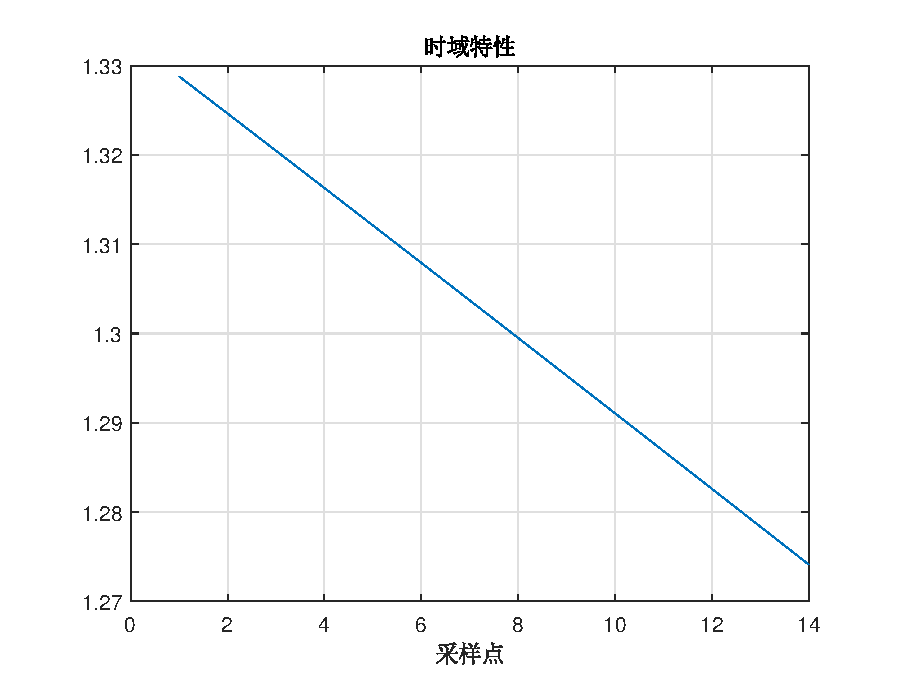
\includegraphics[width = .8\textwidth]{time.eps}
	\caption{时域特性}
\end{figure}
\begin{figure}[H]
	\centering
	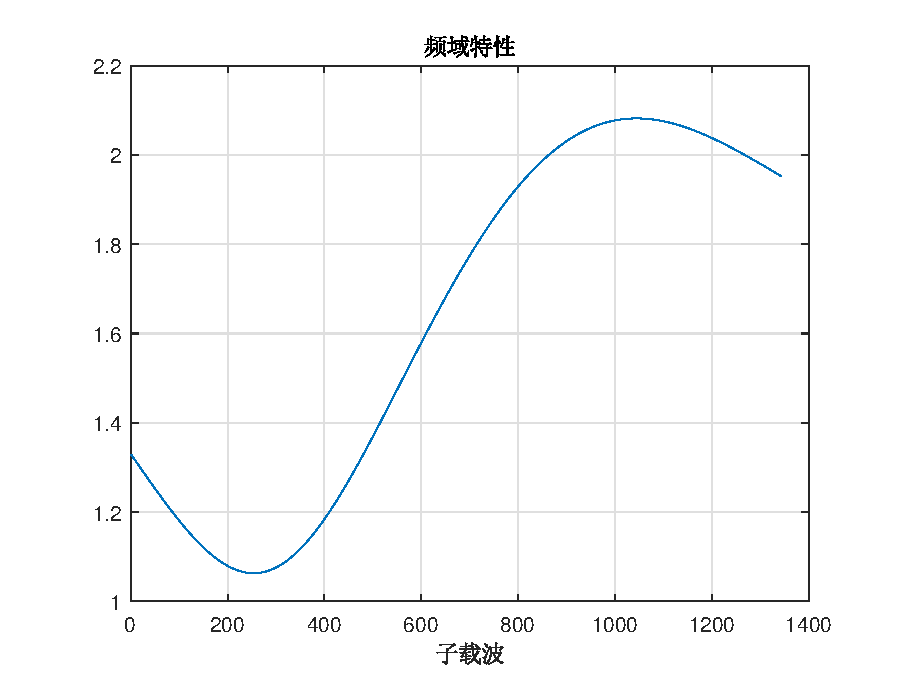
\includegraphics[width = .8\textwidth]{freq.eps}
	\caption{频域特性}
\end{figure}
\begin{figure}[H]
	\centering
	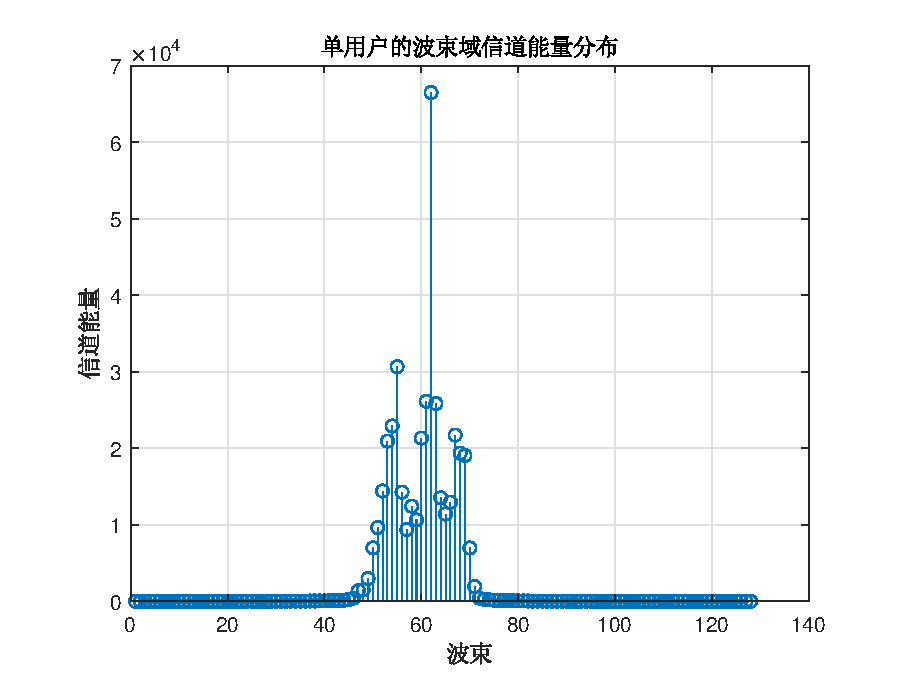
\includegraphics[width = .8\textwidth]{beam.eps}
	\caption{波束域特性}
\end{figure}

%===========第三节=================
\section{处理系统Bug若干}
1. 解包过程中的格式错误;\\
2. 混淆码块分割函数和解码块分割函数;\\
3. 码块分割后未补零。

%===========第四节=================
\section{提高各模块吞吐量}
\subsection{MKL BLAS程序集}
BLAS(Basic Linear Algebra Subprograms,基础线性代数程序集)是一个应用程序接口(API)标准,
用以规范发布基础线性代数操作的数值库(如矢量或矩阵乘法)。
\subsubsection{Level 1:矢量-矢量运算}
$\vec{y}\gets\alpha\vec{x}+\vec{y}$
\subsubsection{Level 2:矩阵-矢量运算}
$\vec{y}\gets\alpha\textbf{A}\vec{x}+\beta\vec{y}$
\subsubsection{Level 3:矩阵-矩阵运算}
$\textbf{C} \gets\alpha\textbf{A}\textbf{B}\vec{x}+\beta\textbf{C}$
\subsection{当前结果}
\subsubsection{8流吞吐量对比}
\begin{figure}[H]
	\centering
	\begin{minipage}[t]{0.4\textwidth}
		\centering
		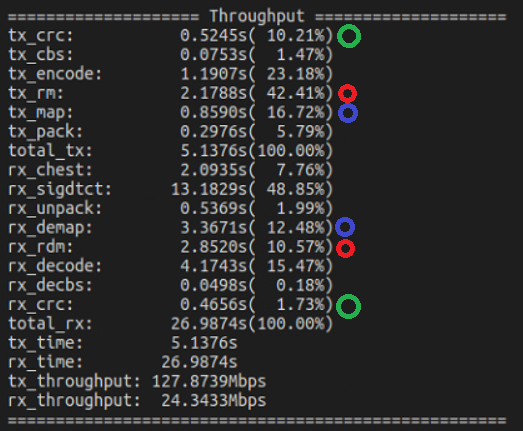
\includegraphics[width = .8\textwidth]{old8.png}
		\caption{优化前}
	\end{minipage}
	\begin{minipage}[t]{0.4\textwidth}
		\centering
		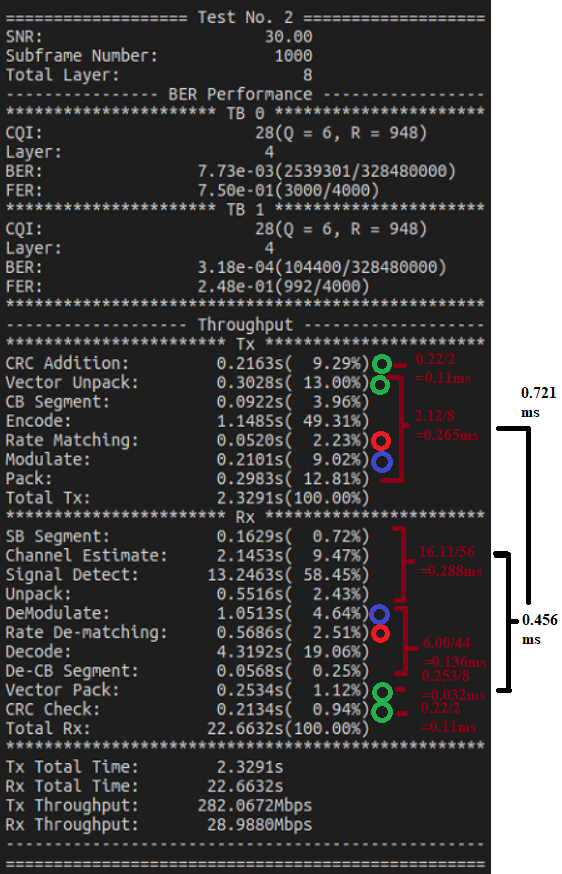
\includegraphics[width = .8\textwidth]{now8.png}
		\caption{优化后}
	\end{minipage}
\end{figure}
\subsubsection{单流结果}
\begin{figure}[H]
	\centering
	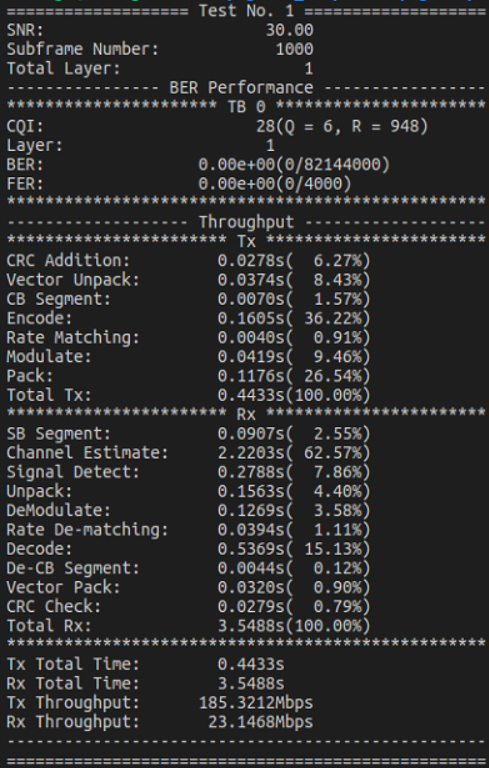
\includegraphics[width = .4\textwidth]{now1.png}
	\caption{单流优化后结果}
\end{figure}

%===========第五节=================
\section{5GNR-LDPC报告}


%===========下周计划=================
% \section{下阶段计划}
% 1. 完善单线程系统(修复Bug)

\end{document}
%%%%%%%%%%%%%%%%%%%%%%%这是正文部分的结束%%%%%%%%%%%%